% Options for packages loaded elsewhere
\PassOptionsToPackage{unicode}{hyperref}
\PassOptionsToPackage{hyphens}{url}
%
\documentclass[
]{article}
\usepackage{amsmath,amssymb}
\usepackage{iftex}
\ifPDFTeX
  \usepackage[T1]{fontenc}
  \usepackage[utf8]{inputenc}
  \usepackage{textcomp} % provide euro and other symbols
\else % if luatex or xetex
  \usepackage{unicode-math} % this also loads fontspec
  \defaultfontfeatures{Scale=MatchLowercase}
  \defaultfontfeatures[\rmfamily]{Ligatures=TeX,Scale=1}
\fi
\usepackage{lmodern}
\ifPDFTeX\else
  % xetex/luatex font selection
\fi
% Use upquote if available, for straight quotes in verbatim environments
\IfFileExists{upquote.sty}{\usepackage{upquote}}{}
\IfFileExists{microtype.sty}{% use microtype if available
  \usepackage[]{microtype}
  \UseMicrotypeSet[protrusion]{basicmath} % disable protrusion for tt fonts
}{}
\makeatletter
\@ifundefined{KOMAClassName}{% if non-KOMA class
  \IfFileExists{parskip.sty}{%
    \usepackage{parskip}
  }{% else
    \setlength{\parindent}{0pt}
    \setlength{\parskip}{6pt plus 2pt minus 1pt}}
}{% if KOMA class
  \KOMAoptions{parskip=half}}
\makeatother
\usepackage{xcolor}
\usepackage[margin=1in]{geometry}
\usepackage{graphicx}
\makeatletter
\def\maxwidth{\ifdim\Gin@nat@width>\linewidth\linewidth\else\Gin@nat@width\fi}
\def\maxheight{\ifdim\Gin@nat@height>\textheight\textheight\else\Gin@nat@height\fi}
\makeatother
% Scale images if necessary, so that they will not overflow the page
% margins by default, and it is still possible to overwrite the defaults
% using explicit options in \includegraphics[width, height, ...]{}
\setkeys{Gin}{width=\maxwidth,height=\maxheight,keepaspectratio}
% Set default figure placement to htbp
\makeatletter
\def\fps@figure{htbp}
\makeatother
\setlength{\emergencystretch}{3em} % prevent overfull lines
\providecommand{\tightlist}{%
  \setlength{\itemsep}{0pt}\setlength{\parskip}{0pt}}
\setcounter{secnumdepth}{-\maxdimen} % remove section numbering
\usepackage{booktabs}
\usepackage{longtable}
\usepackage{array}
\usepackage{multirow}
\usepackage{wrapfig}
\usepackage{float}
\usepackage{colortbl}
\usepackage{pdflscape}
\usepackage{tabu}
\usepackage{threeparttable}
\usepackage{threeparttablex}
\usepackage[normalem]{ulem}
\usepackage{makecell}
\usepackage{xcolor}
\ifLuaTeX
  \usepackage{selnolig}  % disable illegal ligatures
\fi
\IfFileExists{bookmark.sty}{\usepackage{bookmark}}{\usepackage{hyperref}}
\IfFileExists{xurl.sty}{\usepackage{xurl}}{} % add URL line breaks if available
\urlstyle{same}
\hypersetup{
  pdftitle={Report},
  hidelinks,
  pdfcreator={LaTeX via pandoc}}

\title{Report}
\author{}
\date{\vspace{-2.5em}}

\begin{document}
\maketitle

\hypertarget{results}{%
\subsection{Results:}\label{results}}

The ultimate question addressed in this experiment is does the eyespot
`sparkle' decrease the predation rate of lepidoptera. For each
experiment, I used a binomial logit-link generalized linear model to
analyse the effect of design, location, time (collection) and
temperature on the likelihood of predation. All analyses and data
cleaning were carried out in R (ver 4.3.3) with the tidyverse range of
packages (Wickham et al, 2019), car (Fox et al, 2023), patchwork (Lin et
al, 2024) and ggeffects (Lüdecke et al, 2024) packages. Model residuals
were checked with the performance package (Lüdecke et al, 2021). Summary
tables were produced with broom (Robinson et al 2022) and KableExtra
(Zhu, 2020) packages. In the analysis, the term collection refers to the
event of collecting in the models to count predation levels. This
happened 9 times throughout each experiment. Collection is used as a
reference for time into the experiment in analyses and is used as a
numerical variable, so that any potential effects of learning can be
investigated.

\hypertarget{experiment-1}{%
\section{Experiment 1:}\label{experiment-1}}

\hypertarget{influence-of-design-on-predation}{%
\subsection{Influence of Design on
Predation:}\label{influence-of-design-on-predation}}

The main hypothesis of this experiment was that design 3 (2 eyespots)
would show the least amount of predation and design 1 (blank) would show
the greatest likelihood of predation because this pattern is seen in
previous research (). Compared to the blank design, both 1 eyespot
(logit-odds = -1.162 {[}95\% CI: -1.52 - -0.810{]}, z = -6.408, d.f =
1050, P = \textless0.001) and 2 eyespot (logit-odds = -1.335 {[}95\% CI:
-1.69 - -0.985{]}, z = -7.381, d.f = 1050, P = \textless0.001) designs
showed significantly lower log odds likelihood of predation. The size of
these differences is clearer when visualised through probabilities
(Table 1). Blank models showed a mean probability of predation of
84.23\% {[}95\% CI: 80.04 - 87.68\%{]}. Mean probability of predation
for models with 1 eyespot was 62.57\% {[}95\% CI: 56.95-67.87\%{]}, and
the lowest mean probability of predation was 58.43\% for models with 2
eyespots {[}95\% CI: 52.75-63.89\%{]}.

\begin{table}[H]
\centering
\caption{\label{tab:unnamed-chunk-2}Mean Probability of Predation For Each Design}
\fontsize{12}{14}\selectfont
\begin{tabular}[t]{lrrrr}
\toprule
Design & Probability & SE & Lower 95\% CI & Upper 95\% CI\\
\midrule
1 & 0.8423 & 0.0194 & 0.8004 & 0.8768\\
2 & 0.6257 & 0.0279 & 0.5695 & 0.6787\\
3 & 0.5843 & 0.0285 & 0.5275 & 0.6389\\
\bottomrule
\end{tabular}
\end{table}

\textbf{Table 1:} Blank models predated significantly more than eyespot
models. Design 1 (blank), design 2 (1 eyespot), design 3 (2 eyespots).
Values obtained using emmeans function, which analysed a binomial
logit-link generalized linear model, to compare the mean probabilities
of predation across three models types of artificial lepidoptera. The SE
column represents standard error, and lower and upper 95\% confidence
intervals are shown.

\begin{center}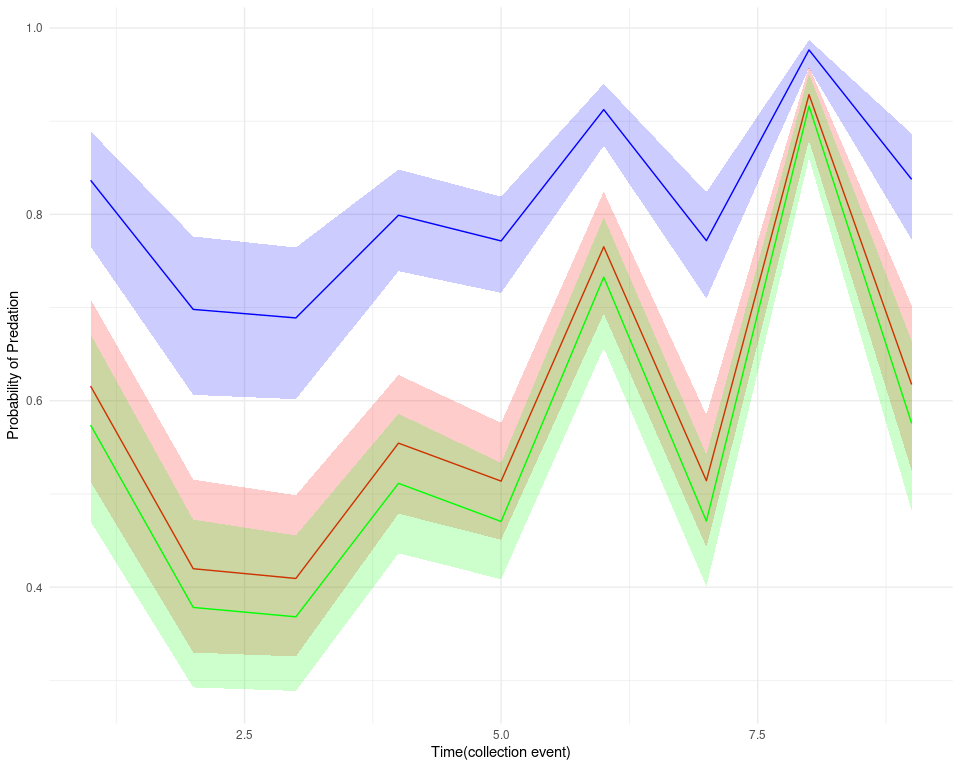
\includegraphics[width=0.8\linewidth]{eyespots_files/figure-latex/unnamed-chunk-4-1} \end{center}

\textbf{Figure 1:} Blank models show greater probability of predation
throughout experiment. Plot shows the probability of predation for three
designs of artificial lepidoptera (blank = blue, 1 eyespot = red, 2
eyespots = green) throughout the experiment. Models were left exposed to
predators in 48 hour periods. Y axis represents the probability of
predation and x axis represents collection (or time into experiment).
Shaded areas reprsent the 95\% confidence intervals for probability
predictions of predation for each design. Probability predictions made
using the augment\_glm function which analysed a binomial logit-link
generalized linear model.

\hypertarget{influence-of-temperature-on-predation}{%
\subsection{Influence of Temperature on
Predation:}\label{influence-of-temperature-on-predation}}

The relationship between temperature and predation rates in birds is
complex and can be influenced by a combination of factors including
metabolic rate, foraging efficiency, breeding behavior, prey behavior,
and habitat availability (Alatalo, R.V., 1982). Model analysis showed a
significant negative relationship between temperature and probability of
predation (logit-odds = -0.210 {[}95\% CI: -0.318 - -0.103{]}, z =
-3.84, df = 1050, P = \textless0.001). Figure 1 shows the relationship
between temperature and predicted probability of predation.

\begin{center}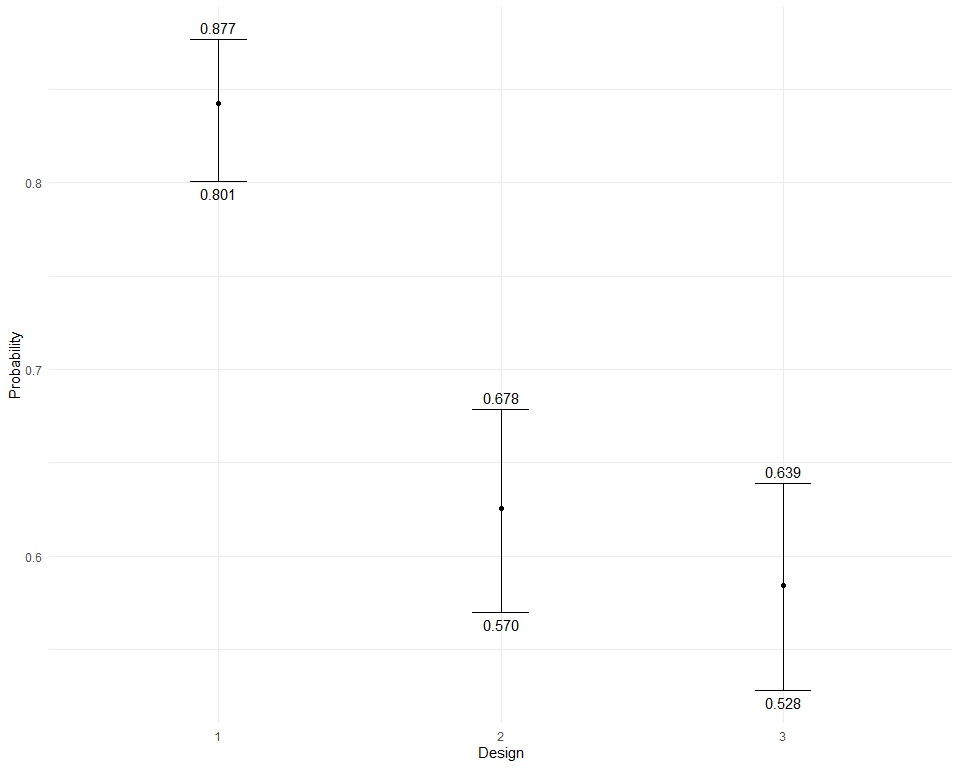
\includegraphics[width=0.8\linewidth]{eyespots_files/figure-latex/unnamed-chunk-5-1} \end{center}

\textbf{Figure 2} Probability of predation decreases with increases in
temperature. Probability of predation decreases from 84\% (95\% CI: 78 -
88\%) at 9 degrees celsius to 69\% (95\% CI: 60 - 76\%) at 13 degrees
celsius. Black line shows this decrease and grey area represents 95\%
confidence intervals of predictions. Y axis represents the predicted
probabilities of predation, obtained using the ggpredict function, which
analysed a binomial logit-link generalized linear model.

\hypertarget{influence-of-location-on-predation}{%
\subsection{Influence of location on
Predation}\label{influence-of-location-on-predation}}

It was hypothesised that, over the whole experiment, the level of
predation between the two locations would follow the same pattern
because predation levels were similar during the preliminary experiment.
Analysis of the model showed that likelihood of predation was
significantly lower in location 2 compared to location 1 (logit-odds:
-1.76 {[}95\% CI: -2.44 - -1.09{]}, z = -5.10, df = 1050, P =
\textless0.001).

\begin{center}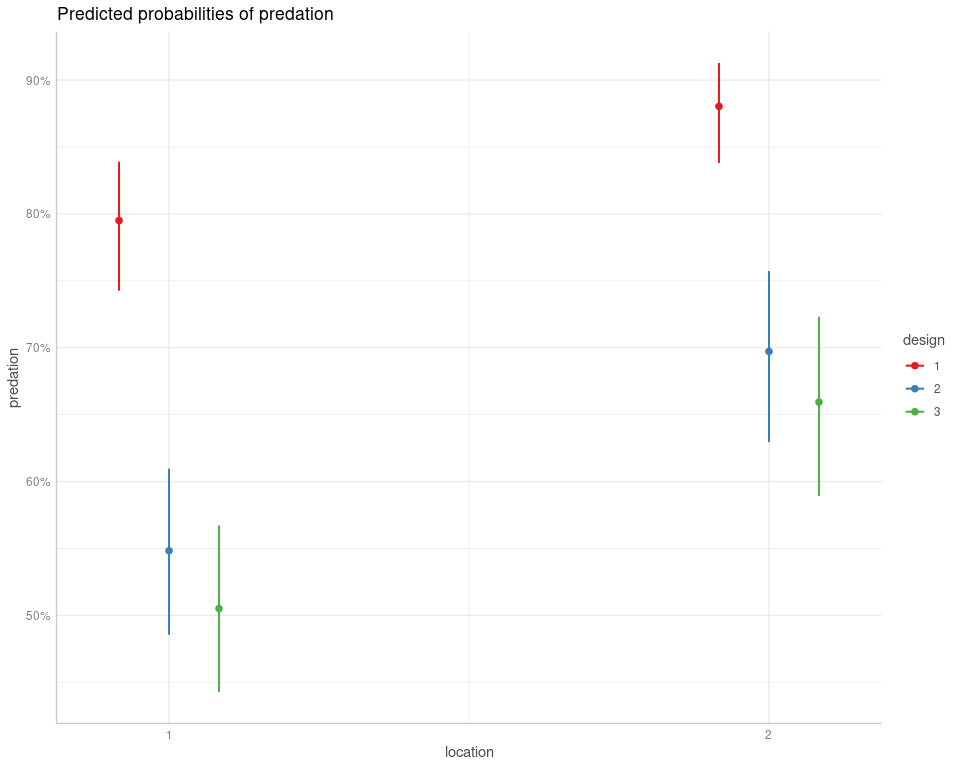
\includegraphics[width=0.8\linewidth]{eyespots_files/figure-latex/unnamed-chunk-6-1} \end{center}

\textbf{Figure 3:} Probability of predation higher for all designs at
location 2. Plot shows probabilities of predation across three designs
of artificial Lepidoptera. Pattern of predation across all three designs
remain similar across both locations but a greater probability of
predation seen at location 2. Upper and lower boundaries for each data
point represent 95\% confidence intervals. Key describes which colours
represent each design. Y axis represents probability of predation and x
axis represents location. Predictions made using the ggpredict function
which analysed a binomial logit-link generalized linear model.

\hypertarget{influence-of-learning-on-predation}{%
\subsection{Influence of Learning on
Predation:}\label{influence-of-learning-on-predation}}

Previous studies have found that over time birds are capable of learning
that the lepidopteran models are fake prey (Blut et al, 2012). It was
hypothesised that the level of predation would increase over the
experimental period because of this. It was plausible that the effects
of learning could be different between the two locations but also
between designs, therefore two interaction terms, one between collection
and location and the other between collection and design, were included.
I found no significant evidence of an interaction between collection and
design (χ² 2,1050 = 3.19, P = 0.2) and this was dropped from the model.
I did find significant evidence of an interaction between collection and
location (χ² 1,1050 = 54.41, P = \textless0.001). I found a significant
positive relationship between collection and probability of predation at
location 2 (logit-odds = 0.480 {[}95\% CI: 0.346 - 0.622{]}, z = 6.831,
d.f = 1050, P = \textless0.001). In contrast, at location 1, the effect
of collection on predation was not statistically significant. This
suggests that learning occurred in birds at location 2 but not location
1.

\begin{center}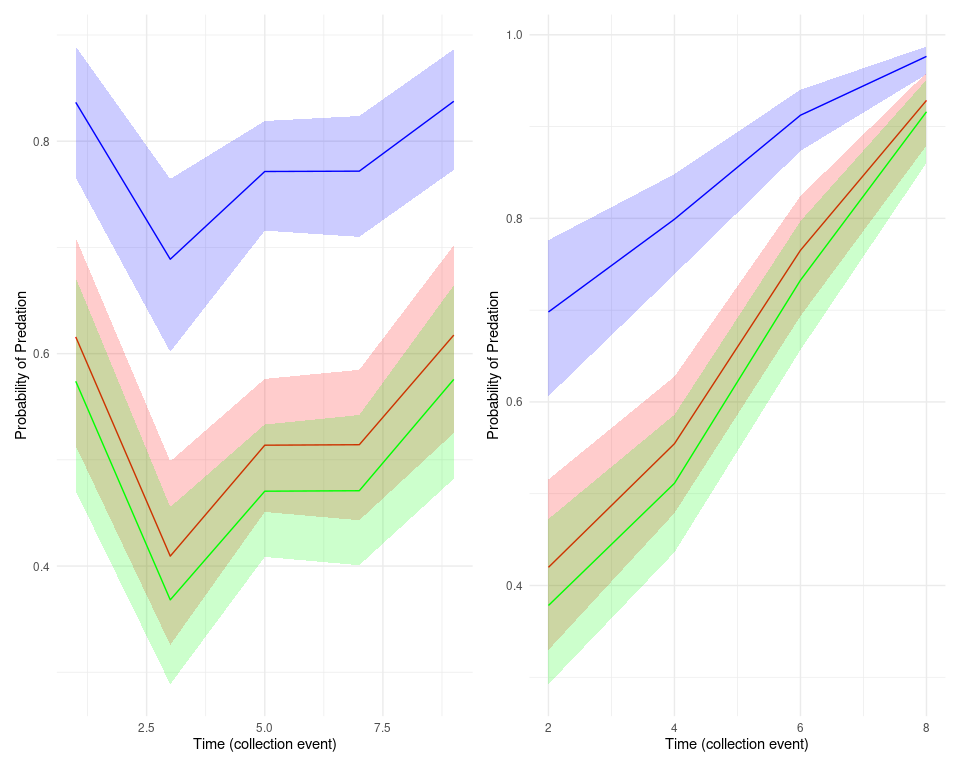
\includegraphics[width=0.8\linewidth]{eyespots_files/figure-latex/unnamed-chunk-7-1} \end{center}

\textbf{Figure 4:} The impact of learning on predation. The plot shows
the relationship between probability of predation and time into the
experiment. Y axis represents probability of predation and x axis
represents collection event number. Blue represents design 1 (blank),
red represents design 2 (1 eyespot) and green represents design 3 (2
eyespots). Artificial Lepidopteran models were exposed to predators in
48 hour periods across 9 collection events. At location 2, predation
levels were significantly influenced by collection (or time into the
experiment). This indicates that learning significantly influenced the
probability of predation at location 2 but not location 1. Despite this,
there is an increase in probability of predation after collection 2 at
location 1. The shaded zones represent the 95\% confidence intervals of
predictions for each design. Predictions were made using the
augment\_glm function which analysed a binomial logit-link generalized
linear model.

\end{document}
